\ifdraft TODO

\chapter{The Ethernet Model}
\label{cha:ethernet}

\section{Sending Ethernet Frames}

TODO tags etc

\section{Receiving Ethernet Frames}

TODO tags etc

\section{Frames}

The INET defines these frames in the \ffilename{EtherFrame.msg} file.
The models supports Ethernet II, 803.2 with LLC header, and 803.3 with LLC and SNAP headers.
The corresponding classes are:
\msgtype{EthernetIIFrame}, \msgtype{EtherFrameWithLlc} and \msgtype{EtherFrameWithSNAP}. They all class
from \msgtype{EtherFrame} which only represents the basic MAC frame with source and
destination addresses. \nedtype{EtherMac} only deals with \msgtype{EtherFrame}s, and does not
care about the specific subclass.

Ethernet frames carry data packets as encapsulated cMessage objects.
Data packets can be of any message type (cMessage or cMessage subclass).

The model encapsulates data packets in Ethernet frames using the \ttt{encapsulate()}
method of cMessage. Encapsulate() updates the length of the Ethernet frame too,
so the model doesn't have to take care of that.

The fields of the Ethernet header are passed in a \cppclass{Ieee802Ctrl}
control structure to the LLC by the network layer.


EtherJam, EtherPadding (interframe gap), EtherPauseFrame?


\section{EtherLlc}

EtherFrameWithLLC

SAP registration

% TODO delete EtherLLC, because LLC without SNAP is not used with IP (no ARP,IPv6 SAP)
% TODO modify EtherEncap to handle EtherFrameWithSNAP frames too (we can not send EtherFrameWithSNAP now)

\subsubsection{\nedtype{EtherLlc} and higher layers}

The \nedtype{EtherLlc} module can serve several applications (higher layer protocols),
and dispatch data to them. Higher layers are identified by DSAP.
See section "Application registration" for more info.

\nedtype{EtherEncap} doesn't have the functionality to dispatch to different
higher layers because in practice it'll always be used with IP.

\subsubsection{Communication between LLC and Higher Layers}

Higher layers (applications or protocols) talk to the \nedtype{EtherLlc} module.

When a higher layer wants to send a packet via Ethernet, it just
passes the data packet (a cMessage or any subclass) to \nedtype{EtherLlc}.
The message kind has to be set to IEEE802CTRL\_DATA.

In general, if \nedtype{EtherLlc} receives a packet from the higher layers,
it interprets the message kind as a command. The commands include
IEEE802CTRL\_DATA (send a frame), IEEE802CTRL\_REGISTER\_DSAP (register highher layer)
IEEE802CTRL\_DEREGISTER\_DSAP (deregister higher layer) and IEEE802CTRL\_SENDPAUSE
(send PAUSE frame) -- see EtherLLC for a more complete list.

The arguments to the command are NOT inside the data packet but
in a "control info" data structure of class \cppclass{Ieee802Ctrl}, attached to
the packet. See controlInfo() method of cMessage (OMNeT++ 3.0).

For example, to send a packet to a given MAC address and protocol
identifier, the application sets the data packet's message kind
to ETH\_DATA ("please send this data packet" command),
fills in the \nedtype{Ieee802Ctrl} structure with the destination MAC address and
the protocol identifier, adds the control info to the message, then sends
the packet to \nedtype{EtherLlc}.

When the command doesn't involve a data packet (e.g.
IEEE802CTRL\_(DE)REGISTER\_DSAP, IEEE802CTRL\_SENDPAUSE), a dummy packet
(empty cMessage) is used.

\subsubsection{Rationale}

The alternative of the above communications would be:

\begin{itemize}
  \item adding the parameters such as destination address into the data
    packet. This would be a poor solution since it would make the
    higher layers specific to the Ethernet model.
  \item encapsulating a data packet into an \textit{interface packet} which
    contains the destination address and other parameters. The
    disadvantages of this approach is the overhead associated with
    creating and destroying the interface packets.
\end{itemize}

Using a control structure is more efficient than the interface packet
approach, because the control structure can be created once inside
the higher layer and be reused for every packet.

It may also appear to be more intuitive in Tkenv because one can observe
data packets travelling between the higher layer and Ethernet
modules -- as opposed to "interface" packets.


\subsubsection{EtherLLC: SAP Registration}

The Ethernet model supports multiple applications or higher layer
protocols.

So that data arriving from the network can be dispatched to the
correct applications (higher layer protocols), applications
have to register themselves in \nedtype{EtherLlc}. The registration
is done with the IEEE802CTRL\_REGISTER\_DSAP command
(see section "Communication between LLC and higher layers")
which associates a SAP with the LLC port. Different applications
have to connect to different ports of \nedtype{EtherLlc}.

The ETHERCTRL\_REGISTER\_DSAP/IEEE802CTRL\_DEREGISTER\_DSAP commands use only the
dsap field in the \cppclass{Ieee802Ctrl} structure.

\section{EtherMac}

The operation of the MAC module can be schematized by the following state chart:

\begin{center}
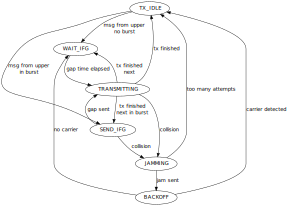
\includegraphics{figures/EtherMAC_txstates}
\end{center}

Unlike \nedtype{EtherMacFullDuplex}, this MAC module processes the incoming packets when their
first bit is received. The end of the reception is calculated by the MAC and
detected by scheduling a self message.

When frames collide the transmission is aborted -- in this case the transmitting
station transmits a jam signal. Jam signals are represented
by a \msgtype{EtherJam} message. The jam message contains the tree identifier
of the frame whose transmission is aborted. When the \nedtype{EtherMac} receives a jam
signal, it knows that the corresponding transmission ended in jamming and have
been aborted. Thus when it receives as many jams as collided frames, it can
be sure that the channel is free again. (Receiving a jam message marks the
beginning of the jam signal, so actually has to wait for the duration of the jamming.)

\section{EtherMacFullDuplex}

Outgoing packets are transmitted according to the following state diagram:

\begin{center}
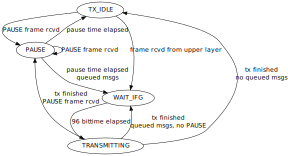
\includegraphics{figures/EtherMACFullDuplex_txstates}
\end{center}

\section{EthernetInterface}

\subsection*{Queueing}

When the transmission line is busy, messages received from the upper layer
needs to be queued.

In routers, MAC relies on an external queue module (see \nedtype{OutputQueue}),
and requests packets from this external queue one-by-one. The name of the
external queue must be given as the \fpar{queueModule} parameer.
There are implementations of \nedtype{OutputQueue} to model finite buffer,
QoS and/or RED.

In hosts, no such queue is used, so MAC contains an internal
queue named \fvar{txQueue} to queue up packets waiting for transmission.
Conceptually, \fvar{txQueue} is of infinite size, but for better diagnostics
one can specify a hard limit in the \fpar{txQueueLimit} parameter -- if this is
exceeded, the simulation stops with an error.

\subsection*{PAUSE handling}
\label{subsec:pause_handling}

The 802.3x standard supports PAUSE frames as a means of flow
control. The frame contains a timer value, expressed as a multiple
of 512 bit-times, that specifies how long the transmitter should
remain quiet. If the receiver becomes uncongested before the
transmitter's pause timer expires, the receiver may elect to send
another PAUSE frame to the transmitter with a timer value of zero,
allowing the transmitter to resume immediately.

\nedtype{EtherMac} will properly respond to PAUSE frames it receives
(\msgtype{EtherPauseFrame} class),
however it will never send a PAUSE frame by itself. (For one thing,
it doesn't have an input buffer that can overflow.)

\nedtype{EtherMac}, however, transmits PAUSE frames received by higher layers,
and \nedtype{EtherLlc} can be instructed by a command to send a PAUSE frame to MAC.

% FIXME PAUSE frames should only be sent on full-duplex ethernet.
%       If a switch uses half-duplex mode to connect to hosts, it can ask sending hosts
%       to slow down their sending rates:
%       - force collisions with incoming frames
%       - make it appear as if the channel is busy
% FIXME PAUSE frames should have 0x8808 in the etherType field

\subsection*{Error handling}

If the MAC is not connected to the network ("cable unplugged"), it will
start up in "disabled" mode. A disabled MAC simply discards any messages
it receives. It is currently not supported to dynamically connect/disconnect
a MAC.

CRC checks are modeled by the \fvar{bitError} flag of the packets. Erronous
packets are dropped by the MAC.


%\subsection*{Auto-Negotiation}
% Ethernet Auto-Negotiation not supported




\fi


